\chapter{Diseño e Implementación} % Main chapter title

\label{Chapter3} % Change X to a consecutive number; for referencing this chapter elsewhere, use \ref{ChapterX}

\definecolor{mygreen}{rgb}{0,0.6,0}
\definecolor{mygray}{rgb}{0.5,0.5,0.5}
\definecolor{mymauve}{rgb}{0.58,0,0.82}

%%%%%%%%%%%%%%%%%%%%%%%%%%%%%%%%%%%%%%%%%%%%%%%%%%%%%%%%%%%%%%%%%%%%%%%%%%%%%
% parámetros para configurar el formato del código en los entornos lstlisting
%%%%%%%%%%%%%%%%%%%%%%%%%%%%%%%%%%%%%%%%%%%%%%%%%%%%%%%%%%%%%%%%%%%%%%%%%%%%%
\lstset{ %
  backgroundcolor=\color{white},   % choose the background color; you must add \usepackage{color} or \usepackage{xcolor}
  basicstyle=\footnotesize,        % the size of the fonts that are used for the code
  breakatwhitespace=false,         % sets if automatic breaks should only happen at whitespace
  breaklines=true,                 % sets automatic line breaking
  captionpos=b,                    % sets the caption-position to bottom
  commentstyle=\color{mygreen},    % comment style
  deletekeywords={...},            % if you want to delete keywords from the given language
  %escapeinside={\%*}{*)},          % if you want to add LaTeX within your code
  %extendedchars=true,              % lets you use non-ASCII characters; for 8-bits encodings only, does not work with UTF-8
  %frame=single,	                % adds a frame around the code
  keepspaces=true,                 % keeps spaces in text, useful for keeping indentation of code (possibly needs columns=flexible)
  keywordstyle=\color{blue},       % keyword style
  language=[ANSI]C,                % the language of the code
  %otherkeywords={*,...},           % if you want to add more keywords to the set
  numbers=left,                    % where to put the line-numbers; possible values are (none, left, right)
  numbersep=5pt,                   % how far the line-numbers are from the code
  numberstyle=\tiny\color{mygray}, % the style that is used for the line-numbers
  rulecolor=\color{black},         % if not set, the frame-color may be changed on line-breaks within not-black text (e.g. comments (green here))
  showspaces=false,                % show spaces everywhere adding particular underscores; it overrides 'showstringspaces'
  showstringspaces=false,          % underline spaces within strings only
  showtabs=false,                  % show tabs within strings adding particular underscores
  stepnumber=1,                    % the step between two line-numbers. If it's 1, each line will be numbered
  stringstyle=\color{mymauve},     % string literal style
  tabsize=2,	                   % sets default tabsize to 2 spaces
  title=\lstname,                  % show the filename of files included with \lstinputlisting; also try caption instead of title
  morecomment=[s]{/*}{*/}
}


%----------------------------------------------------------------------------------------

En este capítulo se explica...

%----------------------------------------------------------------------------------------

\section{Prototipo de pruebas}

El prototipo de pruebas, fue desarrollado con la finalidad de probar todas las funciones de firmware que componen el trabajo y brindar una primera aproximación al prototipo comercial del dispositivo.

Como se vio en la figura 2.1, el dispositivo está compuesto por los siguientes bloques funcionales: microcontrolador, transceptor Wi-Fi, transceptor LoRa, memoria no volátil, reloj en tiempo real y conversor óptico-eléctrico.

La construcción del prototipo de pruebas se realizó en una \textit{breadboard}, para poder realizar cambios en las conexiones de los componentes de una manera sencilla cuando estos se requieran. Se eligieron componentes de hardware acordes con los bloques que constituyen el dispositivo, en su mayor parte módulos de desarrollo con circuitos integrados embebidos que disponen de conectores apropiados para una breadboard. En la figura 3.1 se muestra el diagrama en bloques general con los componentes del prototipo de pruebas.


\begin{figure}[h]
	\centering
	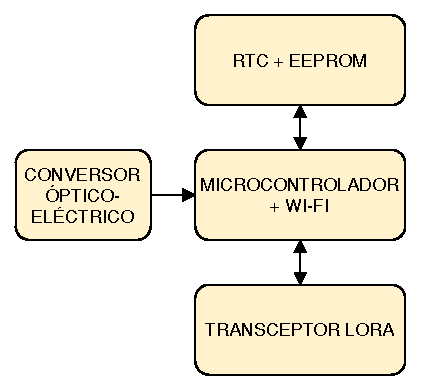
\includegraphics[scale=1]{./Figures/test_blocks.pdf}
	\caption{Diagrama en bloques del prototipo de pruebas.}
	\label{fig:blocksTest}
\end{figure}

Para garantizar un tiempo corto en la obtención de los componentes del prototipo de pruebas, el criterio predominante para la elección de los componentes de cada uno de los bloques fue la disponibilidad en el mercado local. Además, la elección de proveedores locales aseguró la restitución eficaz de los componentes que se malograron durante el desarrollo.

\subsection{Microcontrolador + Wi-Fi}

Este bloque fusiona los bloques microcontrolador y transceptor Wi-Fi. El desarrollo de dispositivos con conexión Wi-Fi ha tenido un gran crecimiento en los últimos años (ref), por lo que los fabricantes de circuitos integrados ofrecen soluciones que integran microcontroladores y transceptores Wi-Fi en un solo encapsulado.

El componente elegido para este bloque es la tarjeta de desarrollo NodeMCU de la firma Amica, basado en el módulo ESP-12F de la firma Ai-Thinker. Las características más atractivas de esta tarjeta en lo referente al desarrollo, son alimentación y programación a través de un puerto micro USB, factor de forma adecuado para ser montado sobre un breadboard e incorporación de LEDs y pulsadores en la misma tarjeta. En la figura 3.2 se muestra la NodeMCU.

\begin{figure}[h]
	\centering
	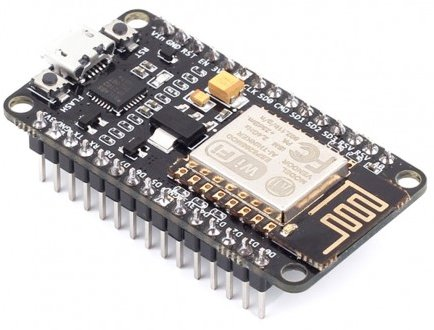
\includegraphics[scale=0.5]{./Figures/nodemcu.jpg}
	\caption{Tarjeta de desarrollo NodeMCU de la firma Amica\protect\footnotemark.}
		\label{fig:cuadradoAzul}
	\end{figure}

	\footnotetext{Imagen tomada de: \url{https://www.amazon.com/-/es/KeeYees-Internet-Development-Wireless-Compatible/dp/B07PR9T5R5}}

El módulo ESP-12F, monta sobre sí un SoC (\textit{System on a Chip}, sistema en un chip) de la firma Espressif Systems, el ESP8266, que funciona como microcontrolador y transceptor Wi.Fi. Otros componentes instalados sobre este módulo son condensadores, resistencias, oscilador, memoria flash y una antena impresa; todos ellos necesarios para que el ESP8266 pueda desempeñar correctamente sus funciones.

El ESP8266 es un chip de bajo costo que incorpora un microcontrolador y un transceptor Wi-Fi, además de contar con un \textit{stack} TCP/IP. Sus características técnicas más relevantes son:
\begin{itemize}
	\item Procesador: Tensilica LX106 de arquitectura RISC(footnote) de 32 bits a una frecuencia de 80 MHz.
	\item RAM: 64 KB para instrucciones y 96 KB para datos.
	\item ROM: externa, puede soportar hasta 16 MB de memoria flash con conexión QSPI(footnote).
	\item Wi-Fi: IEEE 802.11 b/g/n.
	\item Periféricos: GPIO, SPI, I\textsuperscript{2}C, UART y ADC.
\end{itemize}

\subsection{Transceptor LoRa}

La elección del componente de este bloque, 

\subsection{RTC + EEPROM}

Los bloques memoria no volátil y reloj en tiempo real fueron fusionados en un único bloque, ya que comercialmente existen módulos que cumplen ambas funciones. Estos módulos tienen embebidos circuitos integrados de memoria y RTC, además de otros componentes como resistencias, condensadores, osciladores, zócalos para baterías y conectores apropiados para un breadboard. Estos módulos en su gran mayoría poseen una EEPROM como medio de almacenamiento de datos, esta tecnología es preferible sobre las memorias flash en aplicaciones de adquisición de datos, ya que proporciona un número mayor de ciclos de escritura y borrado.

La mayor parte de los módulos que existen en el mercado local cumplen cabalmente con las funciones que requiere este bloque, pero, debido a la cantidad de pines utilizables de la NodeMCU se tuvo preferencia por los módulos que tenían integrados chips con interfaz I\textsuperscript{2}C. Asimismo, al haber muchos módulos que cumplían el requisito de la interfaz, se buscó uno que tuviera un RTC con la capacidad de generar alarmas en función de la hora. En la figura 3.2 se observa el módulo de RTC + EEPROM elegido.

\begin{figure}[h]
	\centering
	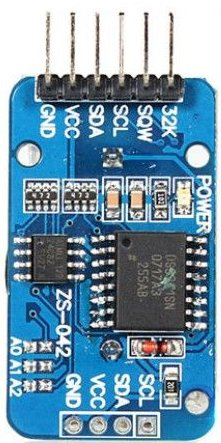
\includegraphics[scale=0.45]{./Figures/rtc_eeprom.jpg}
	\caption{Módulo RTC + EEPROM\protect\footnotemark.}
		\label{fig:cuadradoAzul}
	\end{figure}

	\footnotetext{Imagen tomada de: \url{https://electropeak.com/extremely-accurate-rtc-module}}

Los circuitos integrados que componen el módulo son el DS3231 y el AT24C32, un RTC y una EEPROM, respectivamente. El DS3231 es un RTC de alta precisión de la firma Maxim Integrated, que cuenta con una interfaz I\textsuperscript{2}C para conectarse con otros dispositivos, también tiene la capacidad de generar alarmas y medir la temperatura. El AT24C32 es una EEPROM de la firma Microchip, con interfaz I\textsuperscript{2}C y 32KB de capacidad de almacenamiento.

\subsection{Conversor óptico-eléctrico}

Para este bloque, el componente elegido es un módulo detector de luz, compuesto por un fototransistor PT333-3C de la firma Everlight y un comparador de voltaje LM393 de la firma Texas Instruments. El módulo genera como salida un pulso eléctrico acotado al nivel de voltaje con el que se alimenta, que está determinado por la cantidad de luz incidente y el valor del potenciómetro incluido. En la figura 3.3 se puede observar el módulo.

\begin{figure}[h]
	\centering
	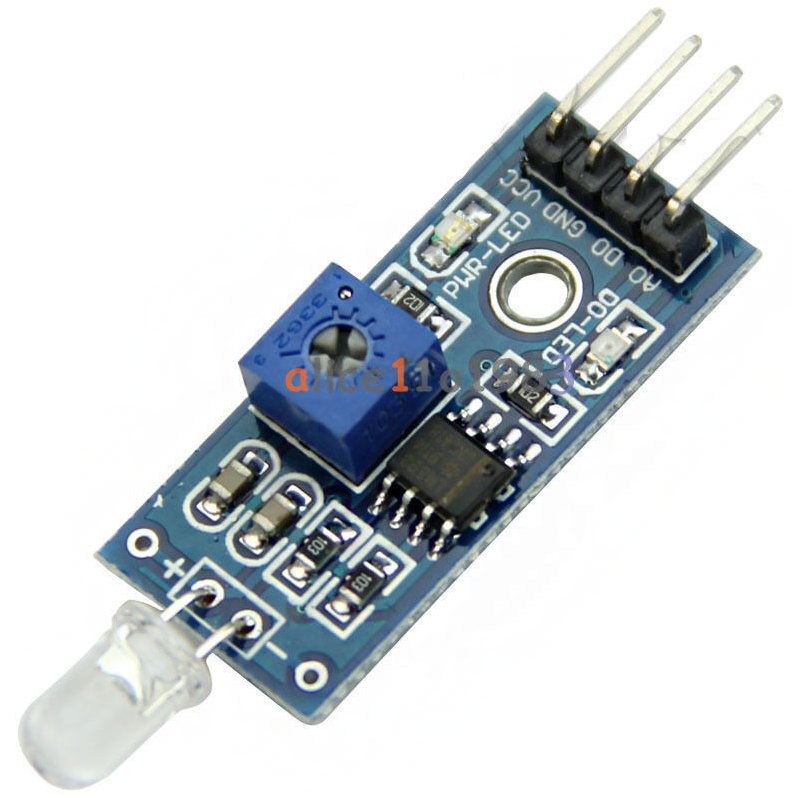
\includegraphics[scale=0.2]{./Figures/coe.jpg}
	\caption{Módulo detector de luz\protect\footnotemark.}
		\label{fig:cuadradoAzul}
\end{figure}

	\footnotetext{Imagen tomada de: \url{https://www.roboter-bausatz.de/en/diy-electronics/extension-modules/sensors/optics-light/149/light-sensor-module}}

%----------------------------------------------------------------------------------------

\section{Diseño de firmware}

El desarrollo del firmware fue la tarea que requirió más esfuerzo en el trabajo, debido a que los objetivos principales del autor fueron lograr modularización y reutilización del código escrito. Para lograr dichos objetivos, el firmware fue estructurado en capas y se utilizó control de versiones para documentarlo. De esta manera, se logró un desarrollo de carácter más profesional que podrá ser reutilizado en futuros proyectos que requieran funciones similares.

Antes de realizar la descomposición del firmware en capas, fue necesario elegir las herramientas de desarrollo implicadas, las mismas fueron imprescindibles al momento de escribir el código fuente del dispositivo. Estas herramientas fueron un SDK (\textit{Software Deveplopment Kit}, kit de desarrollo de software): para proporcionar una API(\textit{Application Programming Interface}, interfaz de programación de aplicaciones) que facilite la escritura de código fuente para el ESP8266 y un IDE (\textit{Integrated Development Enviroment}, Entorno de Desarrollo Integrado) que proporcione funciones para facilitar el desarrollo con el SDK elegido.

\begin{itemize}
	\item ESP8266\_RTOS\_SDK: este SDK fue desarrollado por la firma Espressif Systems para la programación del SoC ESP8266 y facilita un conjunto de funciones para la creación de código fuente. Está basado en el RTOS (\textit{Real-Time Operating System}, sistema operativo en tiempo real) de uso gratuito FreeRTOS (ref), el mismo fue utilizado en las materias sobre sistemas operativos en tiempo real de la Carrera de Especialización y brinda funciones que ayudan a lograr determinismo en la ejecución de las tareas del dispositivo. Asimismo, contiene bastante documentación y ejemplos sobre como utilizar las funciones del ESP8266.
	\item Eclipse: en la documentación de instalación y uso del ESP8266\_RTOS\_SDK (ref), se indica el proceso de configuración de este IDE para compilar el código basado en este SDK. Otro aspecto para su elección fue la experiencia previa del autor con este IDE, el mismo fue utilizado en varias materias de la Carrera de Especialización.
\end{itemize}

Entonces, una vez definidas las herramientas utilizadas, fue posible dividir el firmware en capas, para facilitar el desarrollo y reducir la complejidad del código escrito para el dispositivo. La división en capas del firmware puede observarse en el diagrama de la figura 3.5, donde existen tres capas claramente diferenciadas: SDK, Controladores y Aplicación.

\begin{figure}[h]
	\centering
	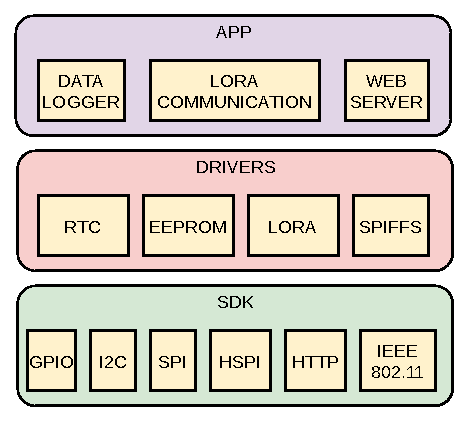
\includegraphics[scale=1]{./Figures/firmware_layers.pdf}
	\caption{Diagrama de capas del firmware.}
		\label{fig:cuadradoAzul}
\end{figure}


\subsection{SDK}

Esta capa está compuesta por la API del SDK y proporciona a las capas de niveles superiores la capacidad de interactuar con los periféricos y protocolos del ESP8266. De todos los periféricos y protocolos que dispone el ESP8266, los que fueron utilizados en el trabajo fueron:

\begin{itemize}
	\item GPIO: este periférico fue utilizado por la capa Aplicación para gestionar los pines disponibles en el ESP8266, ya que algunos de ellos tienen funciones específicas y no pueden ser utilizados para propósitos generales. El SDK posee funciones para definir los pines como entradas o salidas, configuración de interrupciones por flanco positivo o negativo, resistencias de \textit{pull-up} internas, entre otras.
	\item I\textsuperscript{2}C: se utilizó este periférico para que la capa Controladores mediante el protocolo I\textsuperscript{2}C interactúe con el RTC y la EEPROM. Al tener pocos pines disponibles en el ESP8266, este componente se hizo muy importante, ya que para comunicarse con otros circuitos integrados que utilizan el mismo protocolo, solo se necesitan dos pines, uno para datos y otro para el reloj.
	\item SPI: la capa Controladores utiliza este periférico para comunicarse con el transceptor LoRa. El transceptor LoRa elegido, se comunica a través del protocolo SPI con el microcontrolador que lo maneja para intercambiar datos.
	\item HSPI: el ESP8266 no posee memoria ROM embebida en el SoC, por tanto, utiliza una memoria flash externa para almacenar las instrucciones del programa y los datos del usuario. Esta memoria flash se comunica con el ESP8266 mediante el protocolo HSPI. Este periférico se utilizó para que la capa Controladores configurare la flash como un sistema de archivos.
	\item HTTP: el SDK ofrece funciones para ejecutar este protocolo. Fue de utilidad para proporcionar a la capa Aplicación las funciones necesarias para implementar un servidor web.
	\item IEEE 802.11: el ESP8266 tiene embebida toda la electrónica necesaria para implementar los protocolos IEEE 802.11 en sus versiones b, g y n. La capa Aplicación utilizó las funciones disponibles para lograr que el dispositivo funcione como access point y/o estación.
\end{itemize}

\subsection{Controladores}

El ESP8266 está conectado a periféricos de hardware externos, que proporcionan características necesarias para que el dispositivo ejecute eficientemente todas las tareas que debe cumplir. Entonces, el objetivo de esta capa fue desarrollar bibliotecas de firmware para los circuitos integrados externos al ESP8266, que brinden a la capa Aplicación de una interfaz adecuada para comunicarse con ellos. Asimismo, las bibliotecas fueron desarrolladas pensando en ser reutilizadas en futuros proyectos.

Para el manejo de la EEPROM, se desarrolló una biblioteca para que el ESP8266 pueda almacenar y recuperar datos de esta memoria. El elemento más importante en el desarrollo fue el datasheet del AT24C32 (ref), en el mismo se indican todos los pormenores técnicos del funcionamiento de esta EEPROM. Además, se utilizaron las funciones del SDK para gestionar la comunicación I\textsuperscript{2}C en función de la información obtenida del datasheet. Las funciones que proporciona esta biblioteca son:

\begin{itemize}
	\item
	\item
	\item
\end{itemize}

Otra de las bibliotecas desarrolladas fue la que maneja el RTC, que sirvió para configurar la hora, fecha y otras funciones incorporadas. El datasheet del DS3231 (ref), fue la herramienta principal, de este se obtuvo información sobre la dirección de los registros de todas las funciones de este circuito integrado y la forma adecuada de configurarlos. Esto junto con las funciones del SDK referentes al protcolo I\textsuperscript{2}C, permitieron que se disponga de una manera para que el ESP8266 pueda intercambiar datos con el DS3231. En esta biblioteca se desarrollaron las siguientes funciones:

\begin{itemize}
	\item
	\item
\end{itemize}

El desarrollo de la biblioteca para manejar el circuito integrado SX1278, componente central de transceptor LoRa, fue útil para establecer la comunicación de este elemento con el ESP8266, lo que permitió configurar sus parámetros para lograr la transmisión y recepción de datos con otros dispositivos LoRa de manera exitosa. Está basada en la biblioteca Arduino LoRa de Sandeep Mistry (ref) y en el datasheet del SX1278 (ref). Proporciona funciones para:

\begin{itemize}
	\item
	\item
\end{itemize}

Por último, se desarrollo una biblioteca para establecer un sistema de archivos muy reducido llamado SPIFFS (SPI \textit{Flash File System}, sistema de archivos flash SPI), que está albergado en una memoria flash externa, la misma que es utilizada para almacenar el programa grabado en el ESP8266. Esta fue la biblioteca que requirió menos esfuerzo en su desarrollo, debido a que la mayor parte de las funciones estaban disponibles en el SDK. Cumple con las siguientes funciones:
\begin{itemize}
	\item
	\item
\end{itemize}

\subsection{Aplicación}

Esta capa contiene los elementos que permiten al dispositivo ejecutar todas sus tareas correctamente. Está 

%----------------------------------------------------------------------------------------

\section{Interfaz web}

El diseño e implementación de una interfaz web, tiene como objetivo proporcionar a los usuarios, es decir, a los abonados de las compañías eléctricas, la capacidad de interactuar con el dispositivo para visualizar gráficamente información relativa a su consumo eléctrico y configurar parámetros de la conexión Wi-Fi.

Para el desarrollo se utilizo el IDE Visual Studio Code, que ofrece un entorno de desarrollo muy intuitivo y también brinda la posibilidad de descargar \textit{plugins} que facilitan la escritura de código. Asimismo, se utilizaron distintos lenguajes enfocados en el desarrollo web, para brindar a la interfaz una estructura bien definida, estética y funcionalidad. Estos fueron:

\begin{itemize}
	\item HTML: se utilizó para definir todos los aspectos estructurales de la interfaz, como la ubicación de los elementos, las llamadas a bibliotecas externas y otros parámetros informativos. La versión utilizada fue HTML 5.
	\item CSS: brindó control sobre la presentación, formato y el diseño de la interfaz.
	\item JavaScript: permitió dotar de funcionalidad a los elementos de la interfaz. Fue necesaria para realizar el procesamiento de los datos provenientes del dispositivo.
	\item Jquery Mobile: con esta biblioteca fue posible darle a la interfaz un aspecto de aplicación para teléfonos móviles, además de la capacidad de adaptarse a cualquier tamaño de pantalla sin que la información mostrada se vea alterada.
	\item Highcharts: a través de esta biblioteca se logró exhibir la información de consumo eléctrico en un gráfico de barras, de esta manera era más comprensible para el usuario.\end{itemize}

La interfaz web está dividida en dos pantallas, principal y de configuración. La primera es meramente informativa y es donde se muestra el consumo eléctrico al usuario. La segunda permite conectar el dispositivo a un red Wi-Fi existente.

\subsection{Pantalla principal}

Esta pantalla fue diseñada pensando en brindarle al usuario la información de su consumo eléctrico de la manera más simple posible. En la mayor parte del área de la pantalla se muestra un gráfico de barras que presenta el consumo eléctrico de los últimos tres meses y en la esquina superior izquierda un pequeño botón que dirige a la pantalla de configuración.

Al cargar la interfaz en un navegador web, se obtiene mediante el método GET(ref) un archivo CSV (\textit{Comma-Separated Values}, valores separados por coma) con los valores de consumo eléctrico que están almacenados en el dispositivo. Estos son procesados con instrucciones escritas en JavaScript para que la biblioteca Highcharts los utilicé para generar el gráfico de barras. En la figura x se observa la pantalla principal de la interfaz web.

\begin{figure}[h]
	\centering
	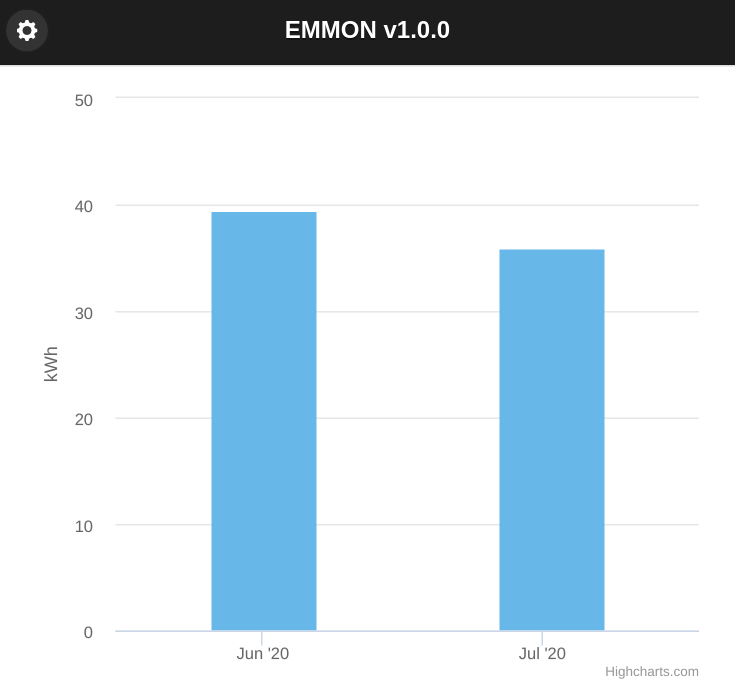
\includegraphics[scale=0.5]{./Figures/interface_main.png}
	\caption{Pantalla principal de la interfaz web.}
	\label{fig:blocksTest}
\end{figure}

\subsection{Pantalla de configuración}

Se diseño esta pantalla para que la única configuración que puede realizarse sea la conexión del dispositivo a una red Wi-Fi existente a través de su SSID y contraseña. Esta pantalla es imprescindible, debido a que el dispositivo no debería ser manipulado manualmente bajo ninguna circunstancia por el usuario.

El componente principal es un formulario para ingresar el SSID y contraseña de la red a la que el usuario desea conectar el dispositivo. En la esquina superior izquierda se encuentra un botón para retornar a la pantalla principal y en la esquina superior derecha un botón para enviar por el método POST el contenido del formulario al dispositivo. En la figura x se muestra la pantalla de configuración de la interfaz web.

\begin{figure}[h]
	\centering
	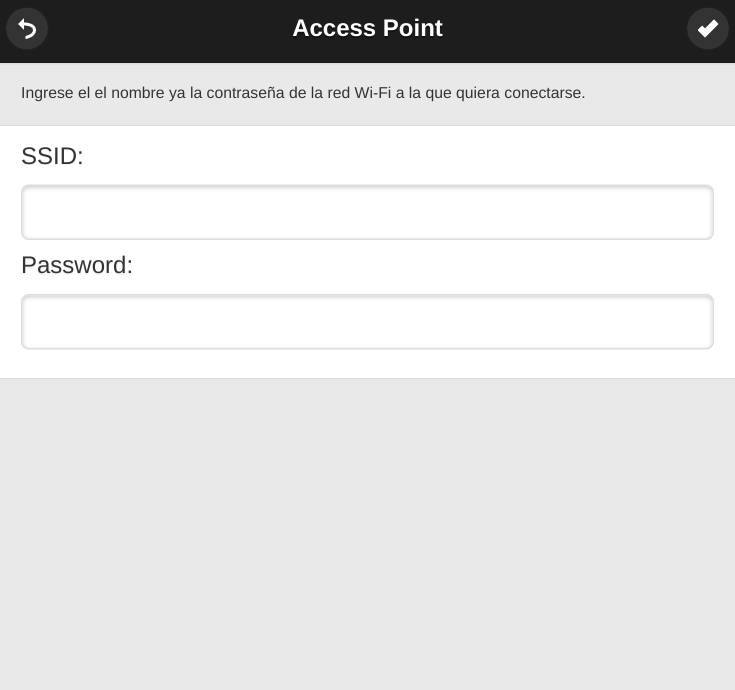
\includegraphics[scale=0.5]{./Figures/interface_conf.png}
	\caption{Pantalla de configuración de la interfaz web.}
	\label{fig:blocksTest}
\end{figure}
%----------------------------------------------------------------------------------------

\section{Prototipo comercial}

El desarrollo de un prototipo para ser comercializado, fue necesario para una primera implementación del dispositivo en un entorno real de trabajo y la realización de pruebas a nivel físico. El mismo consta de una carcasa y un PCB (\textit{Printed Circuit Board}, tarjeta de circuito impreso).

\subsection{Carcasa}

El primer paso, fue elegir una carcasa de dimensiones adecuadas, para que pueda ser montada directamente sobre un medidor de consumo eléctrico domiciliario. Para este fin, se estudió la posibilidad de diseñar una carcasa personalizada, pero, debido a los altos costos de producción a nivel de prototipo, esta idea fue rápidamente descartada. Entonces, después de realizar un análisis de las dimensiones de los medidores utilizados por COPELECT, se eligió una carcasa disponible en el mercado internacional, la VG-S43 de la firma Vange. La elección de esta carcasa sobre otras similares, fue debido a los zócalos que tenía, que se adecuaban perfectamente para que el fototransistor estuviera descubierto y tuviera vista directa con el LED del medidor eléctrico. En la figura x se puede apreciar el carcasa elegida.

\begin{figure}[h]
	\centering
	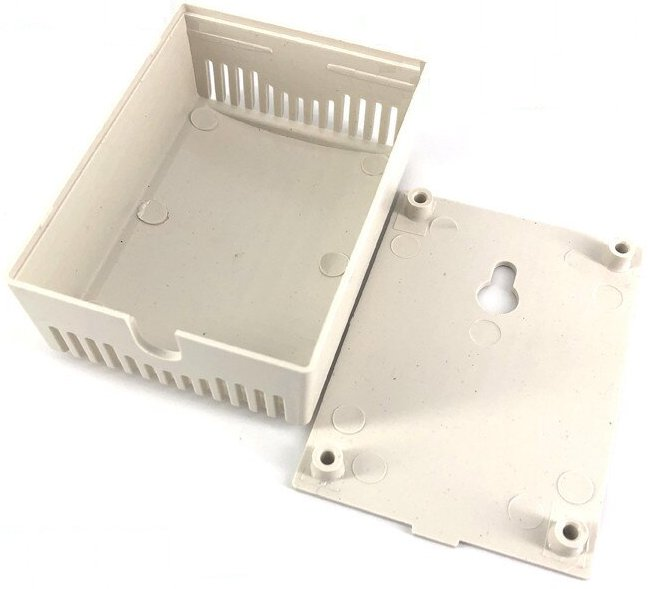
\includegraphics[scale=0.5]{./Figures/case.jpg}
	\caption{Carcasa VG-S43 de la firma Vange\protect\footnotemark.}
		\label{fig:cuadradoAzul}
\end{figure}

	\footnotetext{Imagen tomada de: \url{https://es.aliexpress.com/item/33004284623.html?spm=a2g0o.cart.0.0.50483c00xuS0Xo&mp=1}}

\subsection{Circuito impreso}

Antes de empezar con el diseño del PCB, se realizó la elección de los componentes que serían parte del mismo. En el prototipo de pruebas se utilizaron módulos y tarjetas de desarrollo que con el firmware implementado en ellos, cumplieron todos los requerimientos planteados. Entonces, para que el firmware desarrollado pudiera ser utilizado exitosamente en el prototipo comercial, se utilizaron los circuitos integrados principales de los módulos y tarjetas de desarrollo, también se descartaron los componentes electrónicos que no resultaban necesarios para este trabajo. Existen dos componentes que se implementaron como módulos, el ESP-12F que es componente principal de la NodeMCU, y el RA-01, que es un transceptor LoRa basado en el mismo circuito integrado que el PM1280, el SX1278. Además, el PT333-3C fue sustituido por el PT11-21C, que también es un fototransistor de similares características, pero es un SMD (\textit{Surface-Mount-Device}, dispositivo de montaje superficial).

Una vez elegidos los componentes implicados, se realizó un análisis del consumo de corriente de cada uno de ellos, para implementar una fuente de alimentación adecuada. Cabe resaltar que el voltaje de alimentación de de todos los componentes es 3,3 V. En la tabla x se muestran los valores máximos de consumo de corriente de los componentes, estos datos fueron obtenidos de los \textit{datasheets} de los mismos.

\begin{table}[h]
	\centering
	\caption[Consumo del prototipo comercial]{Tabla de consumo eléctrico de los componentes del prototipo comercial}
	\begin{tabular}{l c}    
		\toprule
		\textbf{Componente} & \textbf{Consumo de corriente (mA)} \\
		\midrule
		ESP-12F 	& 500 (en modo de transmisión continua) \\		
		RA-01		& 93 (en modo transmisor)\\
		DS3231		& 0,2 (en modo activo) \\
		AT24C32 	& 3 (cuando se escribe un dato)\\
		LM393 		& 20 (cortocircuitado a tierra) \\
		PT11-21C	& 20 \\
		\bottomrule
		\hline
	\end{tabular}
	\label{tab:componentsPower}
\end{table}

De la tabla anterior, se determinó que el consumo total de todos los componentes es de 636,2 mA. Al momento de elegir la fuente de alimentación al consumo total se le añadió un margen de seguridad del 50\%, dando un nuevo valor de 954,43 mA. Por lo tanto, la fuente de alimentación elegida debió ser de 3.3 V y 1 A.

Para reducir la cantidad de componentes de la fuente de alimentación, se escogió un módulo conversor de energía alterna a directa. De esta forma, el prototipo comercial podría conectarse directamente a la misma línea eléctrica del medidor. El componente elegido fue el módulo HLK-PM03 de la firma Hi-Link, que proporciona 3,3 V y 1 A a su salida, cuando a la entrada existen 90 V - 240 V alternos. En la figura x puede observarse el módulo para la fuente de alimentación.

\begin{figure}[h]
	\centering
	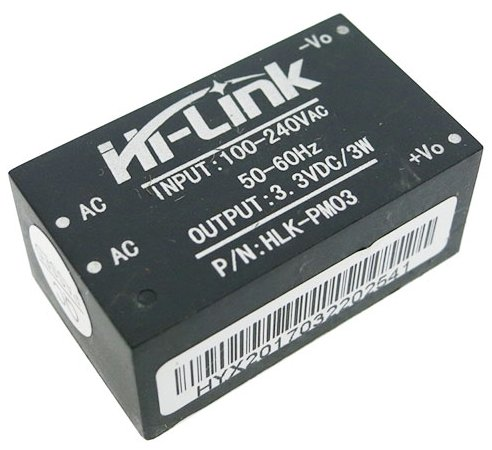
\includegraphics[scale=0.3]{./Figures/acdc_module.jpg}
	\caption{Módulo de alimentación HLK-PM03 de la firma Hi-Link.}
	\label{fig:blocksTest}
\end{figure}

Con ayuda del software KiCAD, se realizó el dibujo de un diagrama esquemático del prototipo comercial, que interconecta todos los componentes y brinda información relacionada a aspectos importantes sobre el funcionamiento y diseño del PCB. En la figura x se muestra el diagrama esquemático del prototipo comercial.

\begin{figure}[h]
	\centering
	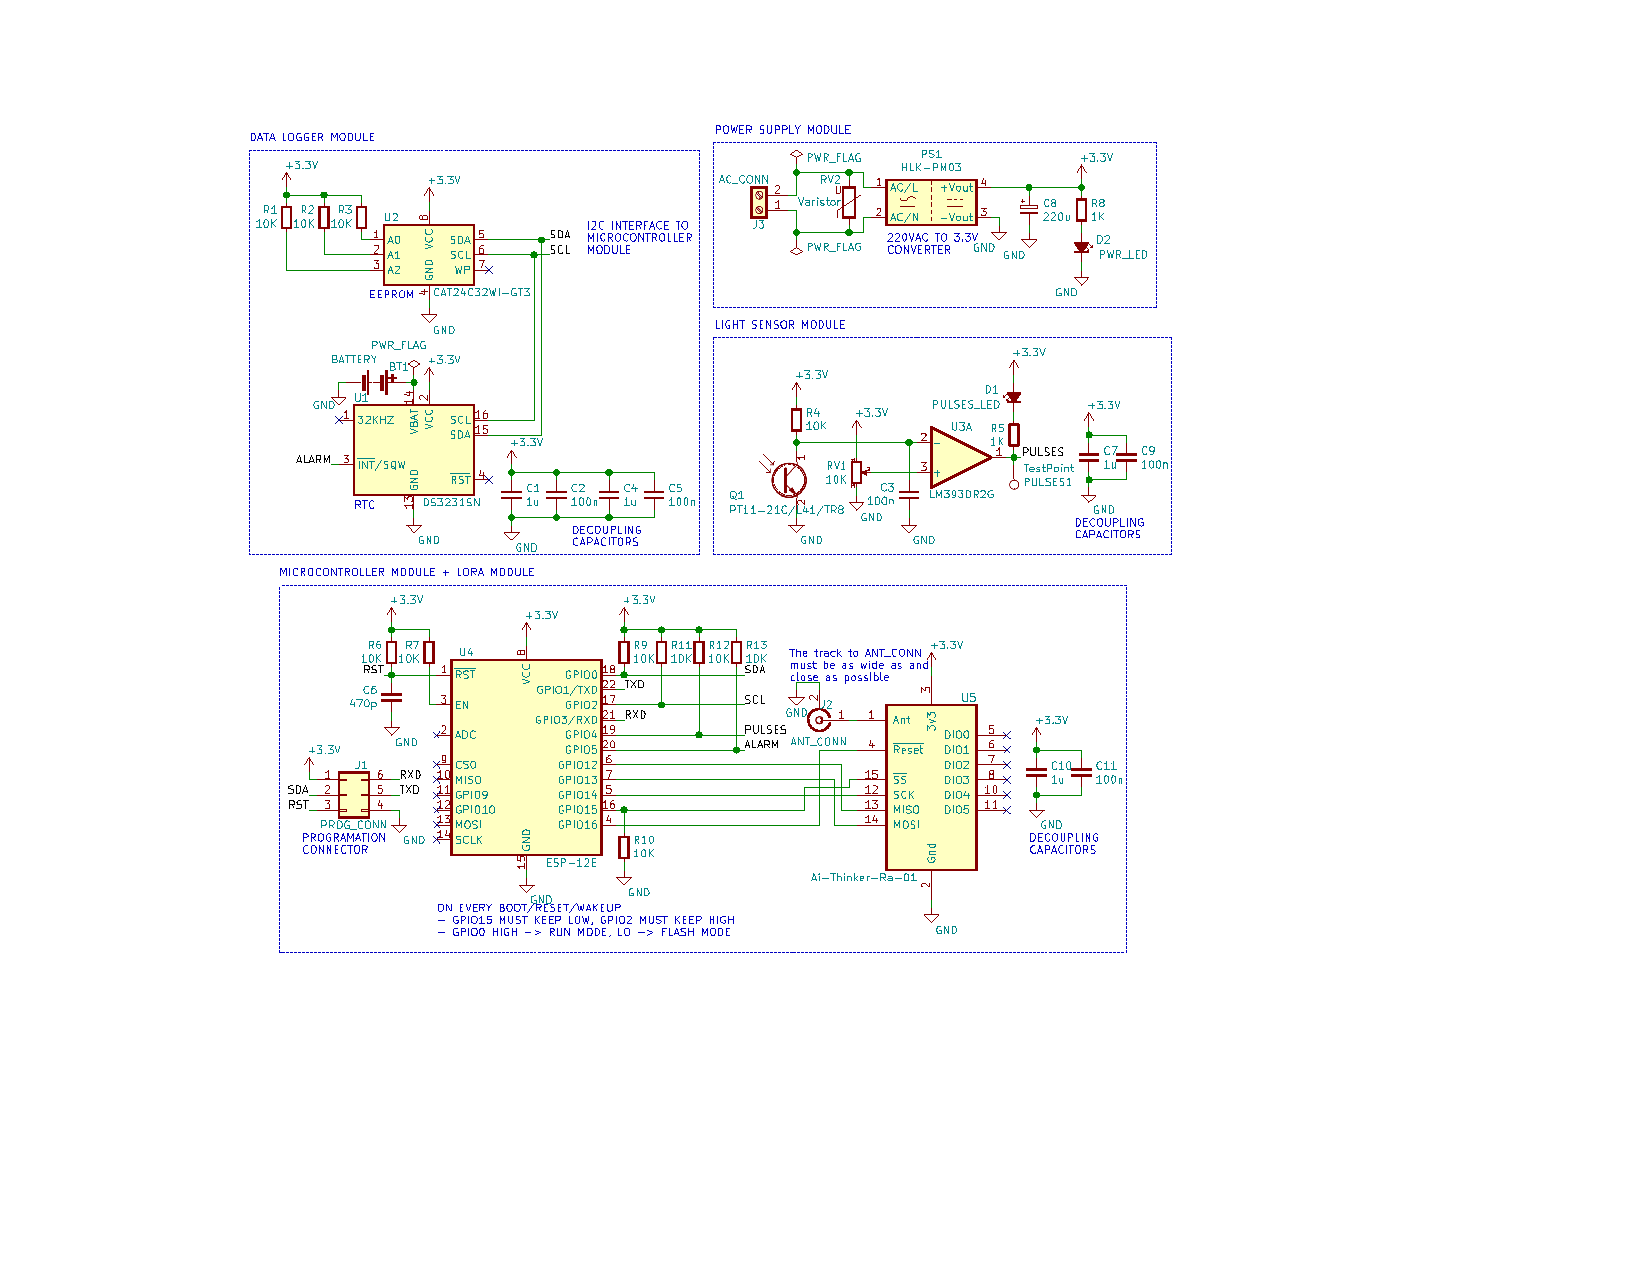
\includegraphics[scale=0.9]{./Figures/schematic.pdf}
	\caption{Diagrama esquemático del prototipo comercial.}
		\label{fig:cuadradoAzul}
\end{figure}

Del diagrama anterior, se puede notar que se añadieron \textit{test points} para poder probar la respuesta del sensor de luz mediante instrumentación especializada. Se añadieron también, un conector destinado a la depuración del código almacenado en el ESP8266, junto con LEDs para monitorear el estado de la fuente y el sensor de luz.

Con el diagrama esquemático finalizado, se realizó la ERC (\textit{Electrical Rule Check}, comprobación de reglas eléctricas) en busca posibles cortocircuitos, conexiones ilegales y contactos flotantes entre otras comprobaciones. Posteriormente, se dibujó el circuito impreso, donde se tuvieron en consideración las restricciones físicas impuestas por la elección de la carcasa. Se tuvo especial énfasis en la ubicación de los conectores, para que estos quedaran al borde del PCB y pudieran ser accedidos con mayor facilidad. El fototransistor quedó ubicado en una posición tal que coincidiera con el zócalo inferior de la carcasa. Otra consideración de importancia fue la distancia entre el transceptor LoRa y el conector coaxial, ambos componentes fueron ubicados muy cerca, de tal forma que la pista que los conectaba tuviera una distancia muy corta, asimismo, se dibujo la pista lo más ancha posible y se pusieron vías conectadas a tierra para lograr una mejor respuesta a las interferencias electromagnéticas.

Las capas \textit{top} y \textit{bottom} del PCB, pueden apreciarse en las figuras x y y, respectivamente. Por otro parte, en las figuras z y a, se muestran el modelo 3D renderizado del PCB y una fotografía del PCB montado.

\begin{figure}[h]
	\centering
	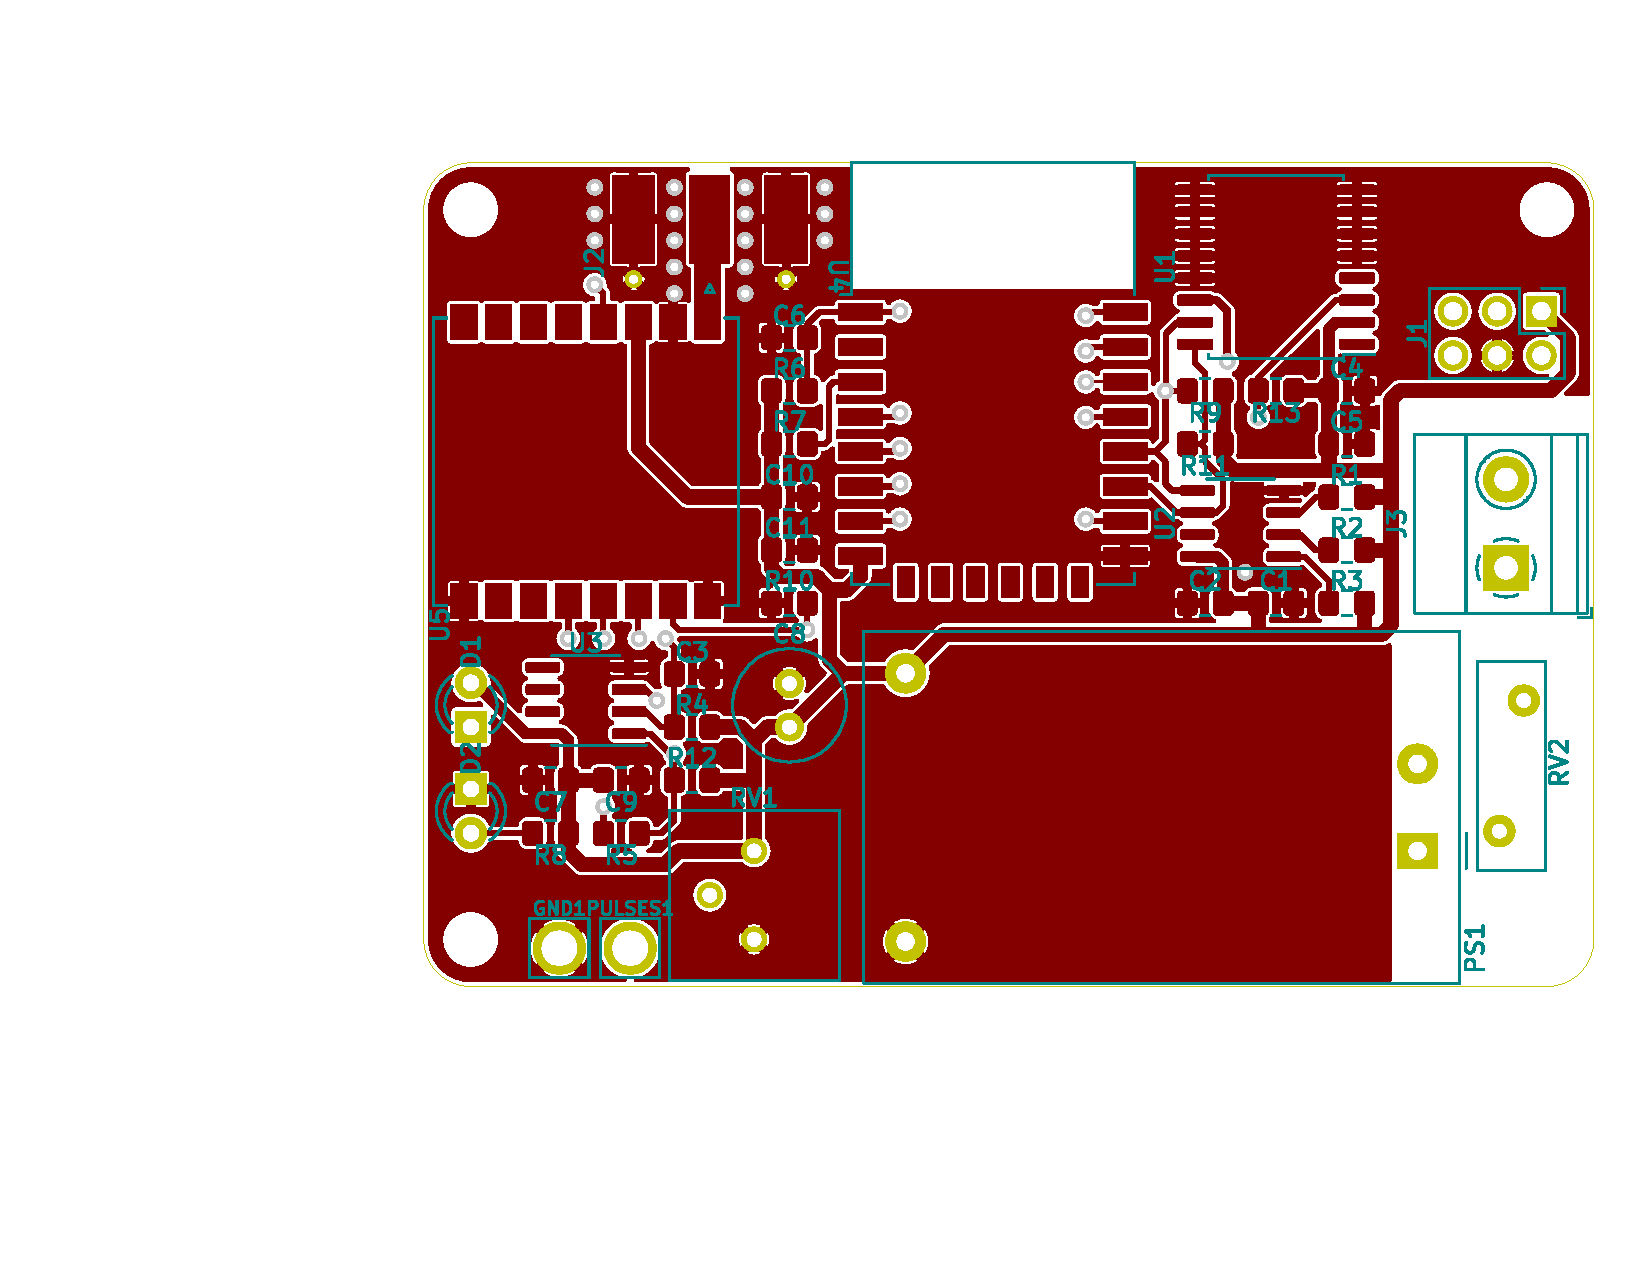
\includegraphics[scale=0.6]{./Figures/pcb_top.pdf}
	\caption{Capa top del PCB.}
		\label{fig:cuadradoAzul}
\end{figure}

\begin{figure}[h]
	\centering
	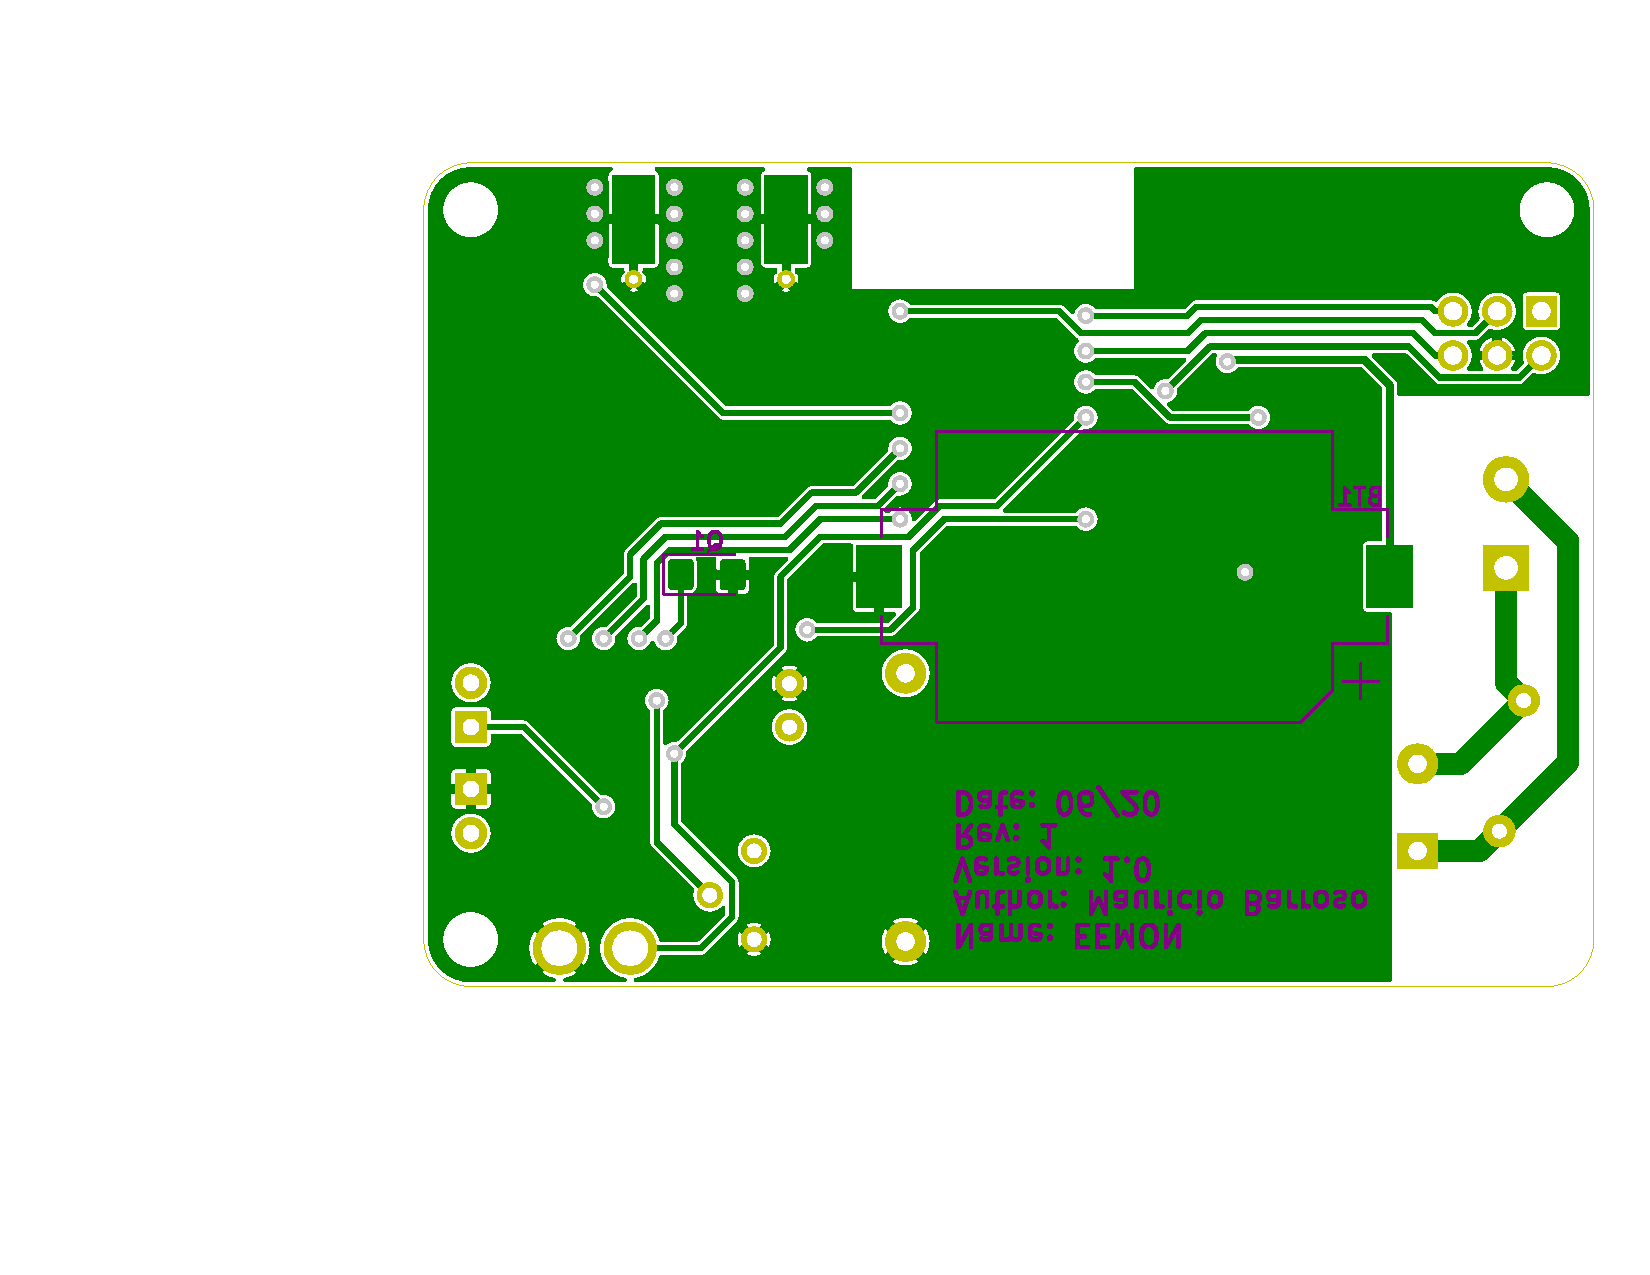
\includegraphics[scale=0.6]{./Figures/pcb_bot.pdf}
	\caption{Capa bottom del PCB.}
		\label{fig:cuadradoAzul}
\end{figure}

\begin{figure}[h]
	\centering
	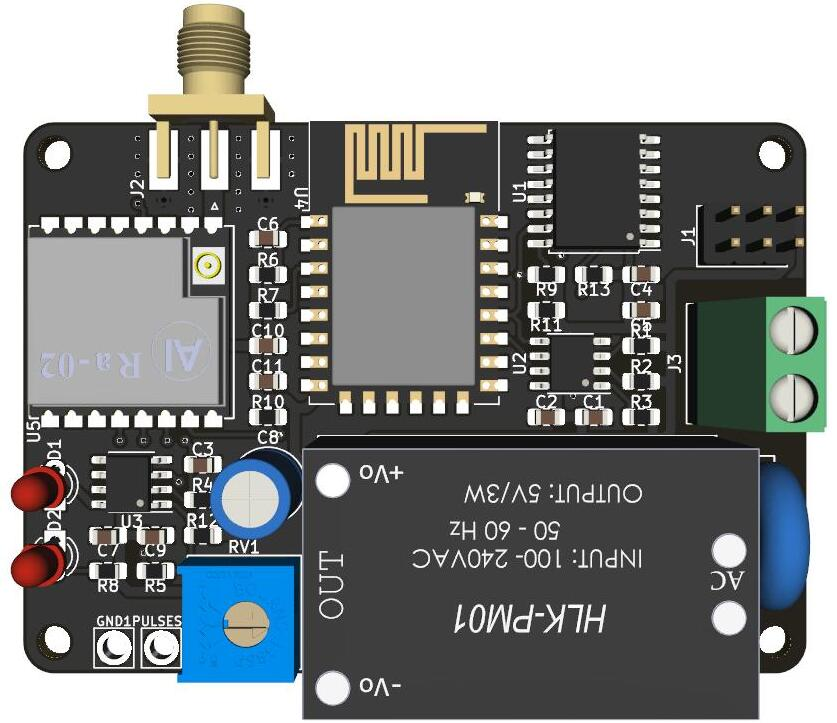
\includegraphics[scale=0.375	]{./Figures/pcb_3d.jpg}
	\caption{Modelo 3D del PCB del prototipo comercial.}
		\label{fig:cuadradoAzul}
\end{figure}

La manufactura del PCB fue realizada por el fabricante JLCPCB y los componentes fueron adquiridos de la firma LCSC. Ambos fueron elegidos por los costos reducidos que ofrecen en sus productos, además de que JLCPCB ofrece el servicio de PCBA (\textit{Printed Circuit Board Assembly}, montaje de PCB) con los componentes que tiene disponibles LCSC.